%%%%%%%%%%%%%%%%%%%%%%%%%%%%%%%%%%%%%%%%%
% University/School Laboratory Report
% LaTeX Template
% Version 3.1 (25/3/14)
%
% This template has been downloaded from:
% http://www.LaTeXTemplates.com
%
% Original author:
% Linux and Unix Users Group at Virginia Tech Wiki 
% (https://vtluug.org/wiki/Example_LaTeX_chem_lab_report)
%
% License:
% CC BY-NC-SA 3.0 (http://creativecommons.org/licenses/by-nc-sa/3.0/)
%
%%%%%%%%%%%%%%%%%%%%%%%%%%%%%%%%%%%%%%%%%

%----------------------------------------------------------------------------------------
%	PACKAGES AND DOCUMENT CONFIGURATIONS
%----------------------------------------------------------------------------------------

\documentclass{article}

\usepackage[version=3]{mhchem} % Package for chemical equation typesetting
\usepackage{siunitx} % Provides the \SI{}{} and \si{} command for typesetting SI units
\usepackage{graphicx} % Required for the inclusion of images
\usepackage{natbib} % Required to change bibliography style to APA
\usepackage{amsmath} % Required for some math elements 
\usepackage[utf8]{inputenc}
\usepackage[margin=1.2in]{geometry}
\usepackage{hyperref}

\setlength\parindent{0pt} % Removes all indentation from paragraphs

% \renewcommand{\labelenumi}{\alph{enumi}.} % Make numbering in the enumerate environment by letter rather than number (e.g. section 6)

\renewcommand{\figurename}{Figura}
\renewcommand{\tablename}{Tabla}
\renewcommand\refname{Referencias}
\def\mean#1{\left< #1 \right>}
%\usepackage{times} % Uncomment to use the Times New Roman font
\renewcommand{\vec}[1]{\mathbf{#1}}

\usepackage{environ}
\NewEnviron{myequation}{%
\begin{equation}
\scalebox{1.1}{$\BODY$}
\end{equation}
}
%----------------------------------------------------------------------------------------
%	DOCUMENT INFORMATION
%----------------------------------------------------------------------------------------

\title{M\'etodos num\'ericos para la Ciencia e Ingenier\'ia \\ Tarea 11: Ajuste de Curvas Bayesiano} % Title

\author{Felipe Toledo B.} % Author name

\date{\today} % Date for the report

\begin{document}

\maketitle % Insert the title, author and date

%----------------------------------------------------------------------------------------
%	SECTION 1
%----------------------------------------------------------------------------------------

\section{Introducción}

En el presente trabajo se estudian modelos orientados a describir una línea de absorción de una observación espectroscópica, presentada en la Figura \ref{fig:datos_originales}.

\begin{figure}[ht]
  \centering
  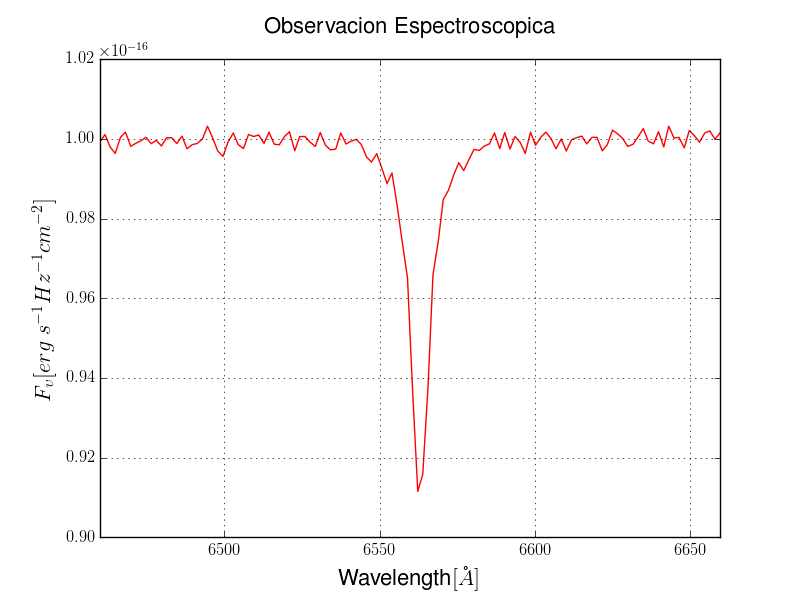
\includegraphics[scale = 0.55]{images/datos_originales.png}
  \caption{Datos originales observados. El nivel del continuo y la longitud de onda central de la línea de absorción son conocidos, con valores $1 \cdot 10^{-16} [\frac{erg}{s\ Hz\ cm^{-2}}]$ y $6563[\AA]$ respectivamente.}
  \label{fig:datos_originales}
\end{figure}

Para describir la línea se probarán dos modelos:

\begin{enumerate}

\item Línea Gaussiana Simple: A partir de la curva se observa que puede resultar conveniente describirla asumiendo que es de forma Gaussiana. En la ecuación (\ref{ec:modelo_1}) se explicita el modelo propuesto. 

\begin{myequation}
M_1(\lambda; A, b) = C_0 - A e^{\frac{(\lambda - \lambda_0)^2}{2 b^2}}
\label{ec:modelo_1}
\end{myequation}

Éste posee dos parámetros libres, $A$ y $b$. El valor de $\lambda_0$ y $C_0$ se asume conocido, donde $\lambda_0$ es la longitud de onda central de la línea de absorción y $C_0$ corresponde al nivel del continuo.  

\item Línea Gaussiana Doble: El modelo está explicitado en la ecuación (\ref{ec:modelo_2}). Se tienen los mismos parámetros conocidos $\lambda_0$ y $C_0$, pero en éste hay cuatro parámetros libres: $A_1$, $A_2$, $b_1$, $b_2$.

\begin{myequation}
M_2(\lambda; A_1, A_2, b_1, b_2) = C_0 - A_1 e^{\frac{(\lambda - \lambda_0)^2}{2 b_1^2}} - A_2 e^{\frac{(\lambda - \lambda_0)^2}{b_2^2}}
\label{ec:modelo_2}
\end{myequation}

\end{enumerate}


% MEJORAR AL FINAL
Los objetivos son estimar el valor de cada parámetro con un intervalo de credibilidad del 68\%, usando métodos Bayesianos , y luego utilizar métodos de selección Bayesiana de modelos para decidir cuál de los dos propuestos representa mejor los datos.


%%%------------------- METODOLOGIA -----------------------------%%%
\section{Metodología}

Para obtener una estimación de los parámetros $\vec{\Theta}$ para cada modelo $M$, se utiliza la regla de Bayes (\ref{eq:bayes}) y los datos empíricos $\vec{x} = (\vec{\lambda}, \vec{F})$.

\begin{myequation}
  P(\Theta| \vec{x}, M) = \frac{P(\vec{x}|\Theta, M) P(\Theta| M)}{P(\vec{x}|M)}
  \label{eq:bayes}
\end{myequation}

El término $P(\Theta| \vec{x}, M)$ indica la probabilidad a posteriori de que los parámetros representen a los datos $\vec{x}$ para el modelo $M$. Se calcula utilizando la distribución de probabilidad de la derecha, donde $P(\vec{x}|\Theta, M)$ es la verosimilitud, que mide la cercanía de los datos respecto a $M(\Theta)$. La probabilidad $P(\Theta| M)$ corresponde a la distribución a priori de los parámetros, la que se fija arbitrariamente. Finalmente, el término $P(\vec{x}|M)$ es difícil de calcular por lo que se utiliza como constante de normalización, de forma que (\ref{eq:bayes}) queda como (\ref{eq:bayes_2}).

\begin{myequation}
  P(\Theta| \vec{x}, M) = K \cdot P(\vec{x}|\Theta, M) P(\Theta| M)
\label{eq:bayes_2}
\end{myequation} 

Para todos los casos se utiliza la función de verosimilitud (\ref{ec:verosimilitud}), donde $M$ representa el modelo a evaluar. El valor de $\sigma$ corresponde al error asociado a cada punto, el cual se estima usando la desviación estándar de los puntos lejanos a la línea de absorción sobre el continuo ($\approx$ error de medición).

\begin{myequation}
  P(\vec{x}|\Theta, M) = \frac{1}{(2 \pi \sigma^2)^{N/2}} e^{\frac{-1}{2 \sigma^2} \sum_{i=1}^N (F_i - M(\lambda_i, \Theta))^2 }
  \label{ec:verosimilitud}
\end{myequation}

La probabilidad a priori de los parámetros de cada distribución dependerá de cada modelo y se detalla en las secciones \ref{sec:modelo1} y \ref{sec:modelo2}. Una vez calculados todos los valores, se procede a calcular la densidad de probabilidad $P(\Theta| \vec{x}, M)$ para una grilla con diversos valores de $\Theta$.

%%%---------------------- PARAMETROS PARA CADA MODELO ---------------------------%%%
\subsection{Parámetros modelo 1: Línea Gaussiana Simple}
\label{sec:modelo1}

El modelo descrito por (\ref{ec:modelo_1}) posee dos parámetros libres, $A$ y $b$. Para utilizar técnicas Bayesianas de estimación es necesario definir una probabilidad a priori para el valor de cada parámetro. Dado que ambos valores están asociados a datos de un fenómeno continuo (mediciones físicas), serán modelados utilizando funciones Gaussianas.

\subsubsection{Parámetro \emph{A}}

A priori se decide que la distribución de $A$ es:

\begin{myequation}
P(A) = \frac{1}{\sqrt{2 \pi} \sigma_A} e^{\frac{(A - \bar A)^2}{2 \sigma_{A}^2}}
\label{ec:distr_A}
\end{myequation}

Para determinar el valor de cada parámetro se debe tener en cuenta que A representa la amplitud en Flujo de la curva Gaussiana del modelo. Para determinarlos se presumirá que las mediciones no están muy alejadas de los valores medios esperados. Con todo esto, se decide lo siguiente:

\begin{itemize}
\item $\bar A$ será la amplitud máxima medida respecto al contínuo.

\item $\sigma_A$ corresponderá al error de medición de Flujo. Se utilizará el mismo valor que el $\sigma$ de la verosimilitud, ya que corresponde al mismo fenómeno.
\end{itemize}

\subsubsection{Parámetro \emph{b}}
Análogamente, la distribución escogida para $b$ es:

\begin{myequation}
P(b) = \frac{1}{\sqrt{2 \pi} \sigma_b} e^{\frac{(b - \bar b)^2}{2 \sigma_{b}^2}}
\end{myequation}

\begin{itemize}
\item $\bar b = 0.8493(\lambda_0 - \lambda(\frac{\bar A}{2}))$

\item $\sigma_b = \frac{\Delta \lambda}{2}$ Se estima a partir de la resolución en longitud de onda (resolución horizontal) del modelo.
\end{itemize}

El valor de $\bar b$ se determina usando la aproximación \emph{Full Width at Half Maximum} (FWHM), donde $\lambda(\frac{\bar A}{2})$ es uno de los valores de longitud de onda en que la línea de absorción cae a la mitad en amplitud\footnote{ Se asume que la línea de absorción es aproximadamente simétrica.}.

\subsection{Parámetros modelo 2: Línea Gaussiana Doble}
\label{sec:modelo2}
En este caso la distribución de probabilidad de cada parámetro también será Gaussiana y de forma análoga a los de la Sección \ref{sec:modelo1}. Entonces, en resumen:

Para las variables $A_1$ y $A_2$:
\begin{itemize}
  \item $\bar{A_1} = \bar{A_2} = \frac{\bar{A}}{2}$ La altura media de la línea de absorción debe ser $\approx \bar{A}$ al sumar las exponenciales.
  
  \item $\sigma_{A_1} = \sigma_{A_2} = \frac{\sigma_A}{2}$ El error en $F$ recibe el mismo escalamiento que $A_1$, $A_2$.
\end{itemize}

Y para $b_1$, $b_2$:

\begin{itemize}
  \item $\bar{b_1} = \bar{b_2} = \bar{b}$ El ancho de la curva se mantiene igual.
  
  \item $\sigma_{b_1} = \sigma_{b_2} = \sigma_b$ El error proviene del mismo fenómeno (es igual).
\end{itemize}

\end{document}
